%
%%As it can be difficult to design controllers for nonlinear systems, compared to linear ones, the model for the inverted pendulum in \autoref{eq:thetaForce} is thus linearized in this section.\\
%%The linearization can be done by several methods, most notably small angle approximation and Taylor expansion. It has been decided to do it by Taylor expansion. 
%The model expression, \autoref{eq:thetaForce}, is expanded to allow linearization of each term individually. This yields \autoref{model_pen}.
%%\begin{align*}
%%\ddot \theta(t)(l\cdot (m_p + m_c)-m_p \cdot l \cdot \cos^2(\theta(t)))&+\dot\theta(t)^2 \cdot (m_p\cdot l\cdot \sin(\theta(t))\cdot \cos(\theta(t)))\nonumber 
%%\end{align*}
%%\vspace{-1.1 cm}
%%\begin{align}
%%&=  \nonumber\\
%%\cos(\theta(t))\cdot F_F(t)+g\cdot& \sin(\theta(t))\cdot (m_p+m_c)
%%\end{align}
%\begin{align*}
%\underbrace{\ddot \theta_p(t) \cdot l(m_p + m_c)\rule[-12pt]{0pt}{5pt}}_{\mbox{1}}
%\underbrace{- \ddot \theta_p(t) \cdot l \cdot \cos^2(\theta(t)) \rule[-12pt]{0pt}{5pt}}_{\mbox{2}}&
%\underbrace{+\dot \theta_p(t)^2 \cdot m_p \cdot l \cdot \sin(\theta_p(t))\cdot \cos(\theta)  \rule[-12pt]{0pt}{5pt}}_{\mbox{3}} \nonumber 
%\end{align*}
%\vspace{-1.1 cm}
%\begin{align*}
%=
%\end{align*}
%\vspace{-1.1 cm}
%\begin{align}
%\underbrace{\cos(\theta_p(t))\cdot F_F(t)\rule[-12pt]{0pt}{5pt}}_{\mbox{4}}
%\underbrace{+ g \cdot \sin(\theta_p(t))\cdot m_p \rule[-12pt]{0pt}{5pt}}_{\mbox{5}}
%\underbrace{+ g\cdot \sin(\theta(t))\cdot m_c \rule[-12pt]{0pt}{5pt}}_{\mbox{6}} \label{model_pen}
%\end{align}
%Note that \autoref{model_pen} is divided into six labeled terms with the purpose to ease traceability in the final linearized equation.\\
%To linearize the model of the inverted pendulum, taylor expansion is applied. The linearization will be done around the segway's equilibrium point, which is when its balanced in an upright position. \\ 
%Linearizing with taylor expansion is simply to approximate a tangent to a given point, in this case at the seqway's equilibrium point, where $\theta_p$ equals zero. Taylor expansion therefore introduces an operating point and a linear deviation around it. These can be expressed as follows.
%%This is the operating point $\bar{\theta}$.
%\begin{equation}
%\theta_p=\bar{\theta}_p+\hat{\theta}_p
%\end{equation}
%\begin{where}
%\va{$\theta_p$}{is the angle of the pendulum}{rad}\\
%\va{$\bar{\theta}_p$}{is the operating point}{rad}\\
%\va{$\hat{\theta}_p$}{is the linear deviation}{rad}
%\end{where}
%\begin{figure}[H]
%\centering
%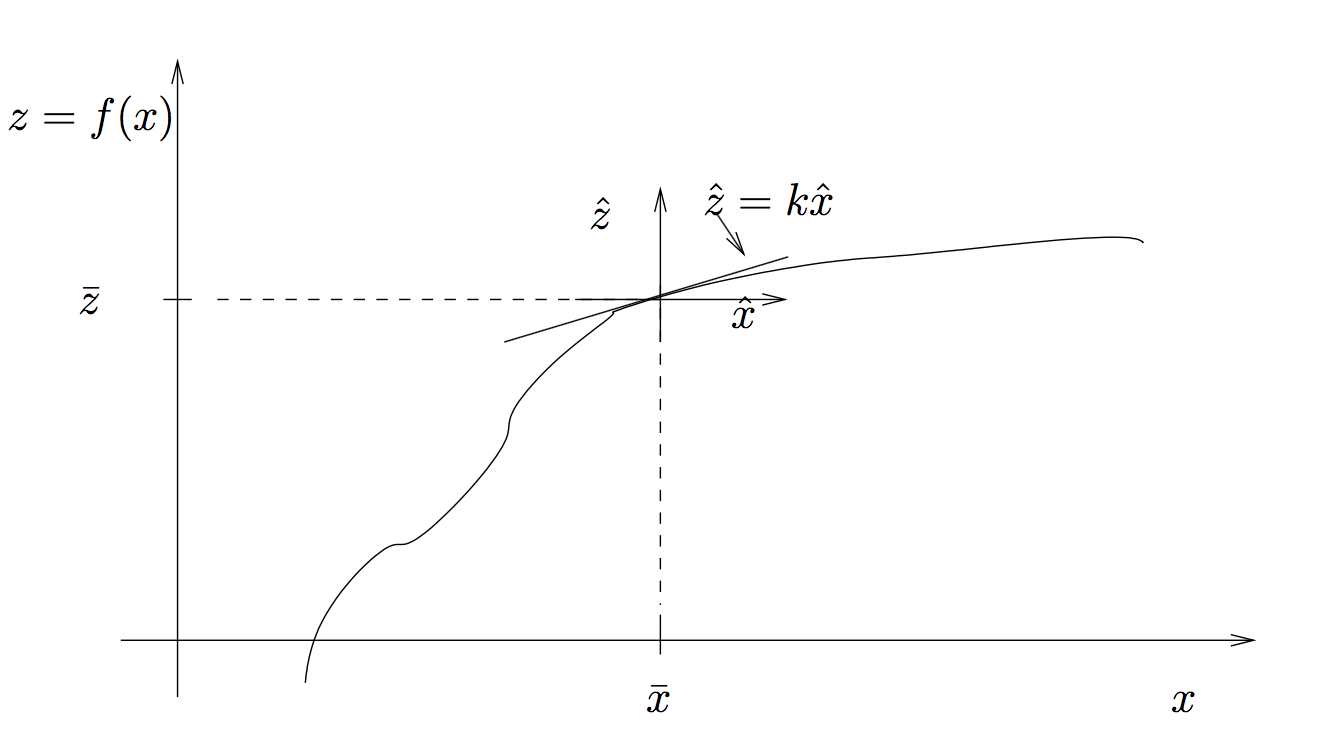
\includegraphics[scale=0.6]{figures/taylor.png}
%\caption{Illustration of the taylor expansion approximation.}
%\label{fig:taylor}
%\end{figure}
%\todo{make figure ourself no source}
%%The model of the inverted pendulum holds $\theta_p$, $\dot{\theta}_p$ and $\ddot{\theta}_$, therefore three differential terms be done for each derivative of $\theta_p$ individually. These are afterwards summed.
%The amount of differential terms in \autoref{eq:taylor} is in this case three as the model of the segway holds $\theta_p$, $\dot\theta_p$ and $\ddot\theta_p$, which shall be linearized. These are afterwards summed.
%
%
%\autoref{eq:taylor} shows the differential terms for the segway's model, but can be extended to fit any nonlinear model expressions.
%%The terms in \autoref{model_pen} will be linearized induvidually before gathered in the final linearized expression for the system's model. \newpar
%%Term 1: \\ 
%%Is already a linear term.\newpar
%%Term 2:
%%\begin{align}
%%\bar{\ddot \theta}(t)\cdot m_p\cdot \cos(\bar{\theta}(t))+m_p\cdot l \cdot \bar{\ddot \theta}(t) \cdot (-2) \cos(\bar{\theta}(t))\cdot \sin(\bar{\theta}(t))\cdot \hat{\theta}(t)+m_p\cdot l \cdot \cos^2(\bar{\theta}(t))\cdot \hat{\ddot \theta}(t)=
%%m_p\cdot l \cdot \cos^2(\bar{\theta}(t))\cdot \hat{\ddot \theta}(t)
%%\end{align}
%%Term 3:
%%\begin{align}
%%\bar{\dot \theta}(t)^2 \cdot m_p \cdot \sin(\bar{\theta}(t))\cdot \cos(\bar{\theta}(t))+\bar{\dot \theta}(t)^2 \cdot m_p \cdot (\cos^2(\bar{\theta}(t))-\sin^2(\bar{\theta}(t)))\cdot \hat{\theta}(t)+2\bar{\dot \theta}(t) \cdot m_p \cdot \sin(\bar{\theta}(t))\cdot \cos(\bar{\theta}(t))=0
%%\end{align}
%%Term 4:
%%\begin{align}
%%\cos(\bar{\theta}(t))\cdot F_F-\sin(\bar{\theta}(t))\cdot F_F\cdot \hat{\theta}(t)=F_F(\cos(\bar{\theta}(t))-\sin(\bar{\theta}(t))\cdot \hat{\theta}(t)
%%\end{align}
%%Term 5:
%%\begin{align}
%%g \cdot \sin(\bar{\theta}(t))\cdot m_p+g\cdot \cos(\bar{\theta}(t))\cdot m_p\cdot \hat{\theta}(t)=g\cdot m_p(\sin(\bar{\theta}(t))+\cos(\bar{\theta}(t))\cdot \hat{\theta}(t))
%%\end{align}
%%Term 6: 
%%\begin{align}
%%g\cdot \sin(\bar{\theta}(t))\cdot m_c+g\cdot \cos(\bar{\theta}(t))\cdot m_c \cdot \hat{\theta}(t)=g\cdot m_c(\sin(\bar{\theta}(t))+\cos(\bar{\theta}(t))\cdot \hat{\theta}(t))
%%\end{align}
%The formular in \autoref{eq:taylor} is applied to each of the six terms individually in the model expression in \autoref{model_pen} to derive a linear aproximation of the inverted pendulum model. This yields the linear approximation:
%\begin{align*}
%\underbrace{\hat{\ddot \theta}_p(t) \cdot l(m_p + m_c)\rule[-12pt]{0pt}{5pt}}_{\mbox{1}}&\underbrace{-m_p\cdot l \cdot \cos^2(\bar{\theta}_p(t))\cdot \hat{\ddot \theta}_p(t)\rule[-12pt]{0pt}{5pt}}_{\mbox{2}}=\underbrace{F_F(t)(\cos(\bar{\theta}_p(t))-\sin(\bar{\theta}_p(t))\rule[-12pt]{0pt}{5pt}}_{\mbox{4}}
%\end{align*}
%\vspace{-1.2 em}
%\begin{align}
%+\underbrace{g\cdot m_p(\sin(\bar{\theta}_p(t))+\cos(\bar{\theta}_p(t))\cdot \hat{\theta}_p(t)) \hat{\theta}_p(t)\rule[-12pt]{0pt}{5pt}}_{\mbox{5}}+&\underbrace{g\cdot m_c(\sin(\bar{\theta}_p(t))+\cos(\bar{\theta}_p(t))\cdot \hat{\theta}_p(t))\rule[-12pt]{0pt}{5pt}}_{\mbox{6}}\label{eq:linear_pen_final}
%\end{align}
%Note that the third term from \autoref{model_pen} equals zero when linearized. This is due to the fact, that this term only holds the operating point, which is zero, as the model is linearized at the seqways equilibrium point. \\\\
%%Based on \autoref{eq:linear_pen_final} a transfer function can be found. The transfer function for the inverted pendulum shall be merged with a transfer function for the motor and wheels model to allow design and implementation of a controller. \\\\
%Having the transfer function in the s-domain allows classical control design methods compared to the time-domain. Laplace transform is performed for this transformation. \\
%Note: $\bar{\theta}_p=0, \hat{\theta}_p=\theta_p$
%\begin{align}
%s^2\cdot \theta_p(s)\cdot l\cdot (m_p+m_c)-m_p\cdot l\cdot s^2\cdot \theta_p(s)&=F_F(s)+ g\cdot m_p\cdot \theta_p(s)+g\cdot m_c\cdot \theta_p(s)\nonumber\\
%\Rightarrow\frac{\theta_p(s)}{F_F(s)}=\frac{1}{s^2\cdot l\cdot m_c-g\cdot (m_p+m_c)}
%&\Rightarrow\frac{\frac{1}{l\cdot m_c}}{s^2-\frac{g\cdot (m_p+m_c)}{l\cdot m_c}}
%\end{align}
%Another method of linearizing is small angle approximation, which is only appropriate to apply when the angle is fairly small, thus the name of this linearization method. \\
%Truncations:
%\begin{align*}
% &\sin{\theta}=\theta\\
 %&\cos{\theta}=1-\frac{\theta^2}{2}\\
 %&\tan{\theta}=\theta \hspace{1 cm}\text{where $\theta$ is in radians}
%\end{align*}
%The linearization is done around the equillibrium, where the angle, $\theta$, is zero. 
%With \autoref{model_pen} as startingpoint, as with the taylor expansion, the small angle approximation is done. Note that Laplace transform is performed as well in the following steps.